\documentclass[a4j,12pt,]{jarticle}
 \usepackage[dvipdfmx]{graphicx}
 \usepackage{float}
 \usepackage{siunitx} %%SI単位系用
 \usepackage{amssymb, amsmath}
 \usepackage{ascmac,here,txfonts,txfonts}
\usepackage{listings,jlisting}
\usepackage[dvipdfmx]{color}
\lstset{%
  language={Python},
  basicstyle={\small},%
  identifierstyle={\small},%
  commentstyle={\small\itshape\color[rgb]{0,0.5,0}},%
  keywordstyle={\small\bfseries\color[rgb]{0,0,1}},%
  ndkeywordstyle={\small},%
  stringstyle={\small\ttfamily\color[rgb]{1,0,1}},
  frame={tb},
  breaklines=true,
  columns=[l]{fullflexible},%
  numbers=left,%
  xrightmargin=0zw,%
  xleftmargin=3zw,%
  numberstyle={\scriptsize},%
  stepnumber=1,
  numbersep=1zw,%
  lineskip=-0.5ex%
}
\begin{document}

{\noindent\small 第16回報告書 \hfill\today}
\begin{center}
  {\Large 分布定数線路の周波数特性}
\end{center}
\begin{flushright}
  愛媛大学工学部 \\
  8531037m \\
  祖父江匠真 \\
\end{flushright}

\section{はじめに}

今回は, ケーブルをマッチング, もしくはマッチングせず受電端側を短絡, 開放した回路における周波数特性を調べたので報告する.

\section{分布定数線路の周波数特性}

伝達関数の計算には, 図\ref{p1}に分布定数線路のF行列

\large
\[
  \left(
  \begin{array}{cc}
      A & B \\
      C & D
    \end{array}
  \right) =
  \left(
  \begin{array}{cc}
      \cosh\gamma l             & Z_0\sinh\gamma l \\
      \frac{\sinh\gamma l}{Z_0} & \cosh\gamma l
    \end{array}
  \right)
\]
\normalsize

と, $R_1 = 0$[Ω]を代入して求めた

\large
\begin{eqnarray}
  G(f) =  \frac{1}{\cosh\gamma l + \frac{Z_0\sinh\gamma l}{R_2}}
\end{eqnarray}
\normalsize

を使用した.

また, $R_2$は, マッチングした場合, マッチングせず受電端側を短絡した場合, 開放した場合でそれぞれ, 50[Ω], 0[Ω], $1.0 × 10^{6}$[Ω]とし, ケーブルの特性インピーダンスは$Z_0 = 50(Ω)$として計算した.

$\gamma$ は
\begin{eqnarray}
  \gamma =  \sqrt{(R + j\omega L)(G + j\omega C)}
\end{eqnarray}
から求めた.
$\gamma$を計算する際の回路素子の値について, Cの値はC = $1.0 × 10^{-10}$[F/m]とし, Lは特性インピーダンス$Z_0$とCを用いて

\large
\begin{eqnarray}
  Z_0 =  \sqrt{\frac{L}{C}}
\end{eqnarray}
\normalsize

より, L = $2.5 × 10^{-7}$ [H/m]とした.

また, R, GについてはR = 0 [Ω/m], G = 0 [S/m]とし, ケーブル長である$l$は, $l = 1000$[m]として計算した.

\begin{figure}[H]
  \begin{center}
    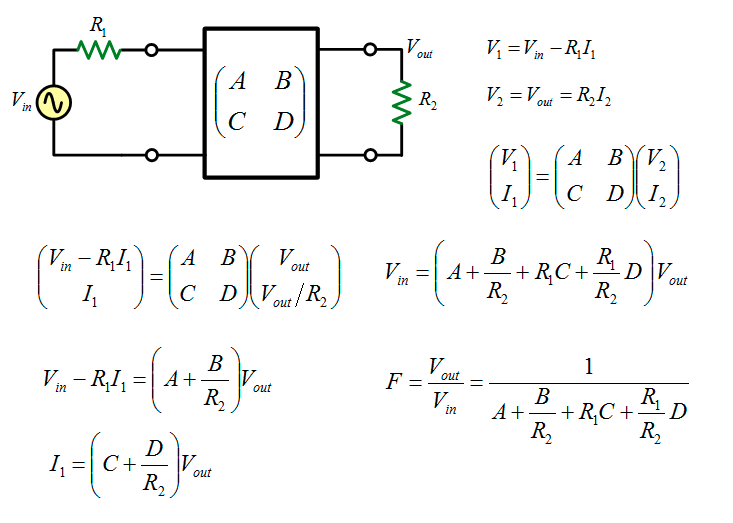
\includegraphics[width=140mm]{transfer.png}
    \caption{F行列から伝達関数を導出する過程}
    \label{p1}
  \end{center}
\end{figure}

以上の条件において, ケーブルをマッチング, もしくはマッチングせず受電端側を短絡, 開放した場合に求めた周波数特性を図\ref{p2}, \ref{p3}, \ref{p4}に示す.

\begin{figure}[H]
  \begin{center}
    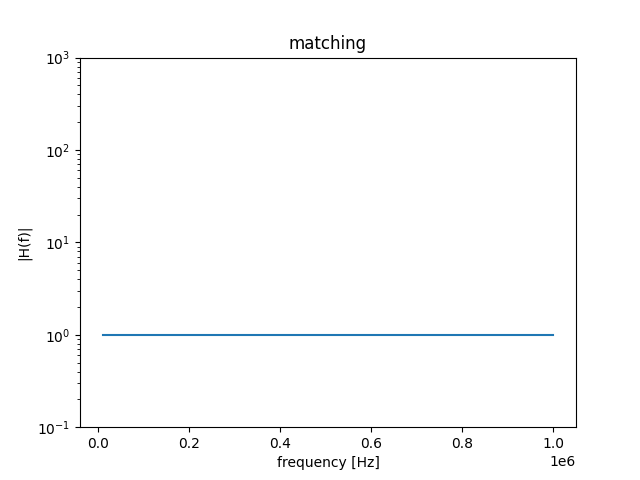
\includegraphics[width=160mm]{matching.png}
    \caption{マッチングした場合における周波数特性}
    \label{p2}
  \end{center}
\end{figure}

\begin{figure}[H]
  \begin{center}
    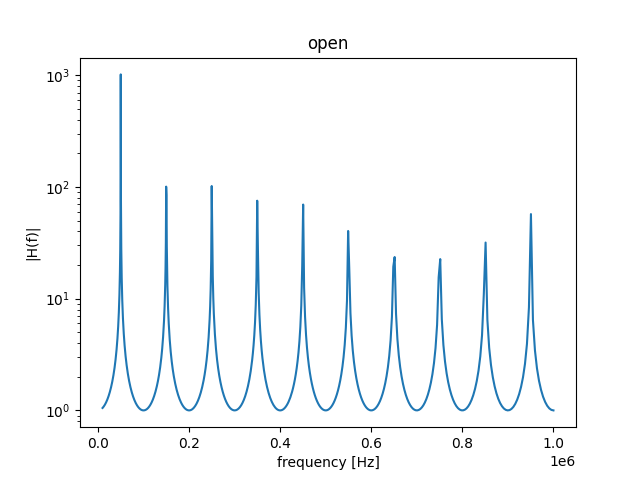
\includegraphics[width=160mm]{open.png}
    \caption{マッチングせず受電端側を短絡した場合における周波数特性}
    \label{p3}
  \end{center}
\end{figure}

\begin{figure}[H]
  \begin{center}
    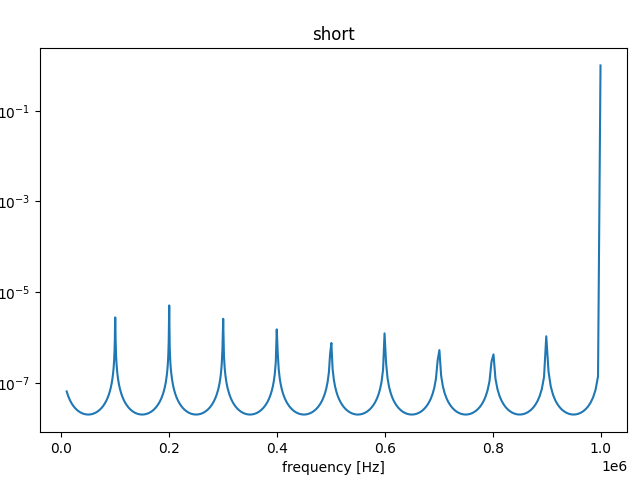
\includegraphics[width=160mm]{short.png}
    \caption{マッチングせず受電端側を開放した場合における周波数特性}
    \label{p4}
  \end{center}
\end{figure}

\section{おわりに}

今回は, ケーブルをマッチング, もしくはマッチングせず受電端側を短絡, 開放した回路における周波数特性を調べた.
マッチングせず受電端側を短絡, 開放した場合において, 周波数特性が周期的に繰り返すようなグラフになったのは, マッチングしなかったことにより反射波が生じたためであると考えられる.

\begin{thebibliography}{5}
  \bibitem{1}都築,”2020Q4-応用通信工学II-都築”, moodle内,参照 December 14,2021.
\end{thebibliography}

\end{document}